% 第 4 章 §4.4 前段（印刷页 200–206）
% 对应 工程文件/work/en/ch04.txt 第 2203–2634 行：图 4.1、§4.4、§4.4.1、§4.4.2、
% §4.4.3 前段（至 (4.54)）。本章唯一的插图在此；编号公式 (4.47)–(4.54)。

% ---------- 图 4.1（全章唯一插图；印刷页 200 / PDF 210） ----------
\setcounter{figure}{0}
\begin{figure}[htbp]
\centering
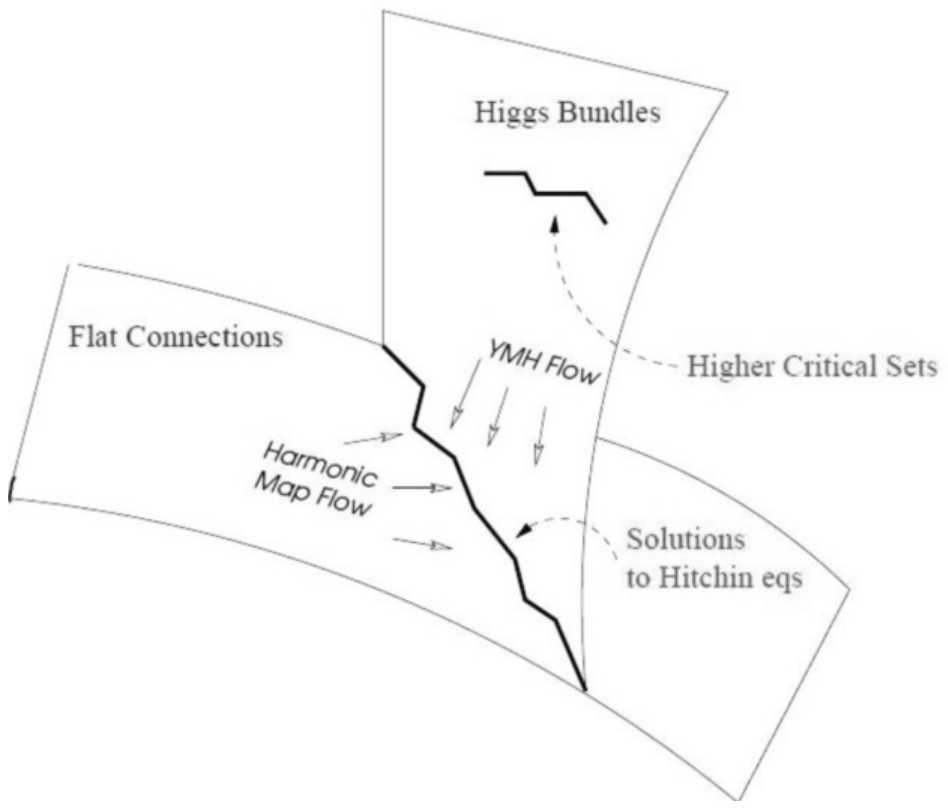
\includegraphics[width=250.3pt]{figs/f4-01.png}
\caption{Higgs 丛与平坦连接。}
\label{fig:4.1}
\end{figure}

\section{微分方程}

\subsection{单值化}

关于本节的讨论，更多内容请参见经典著作 Gunning [28]。

\begin{definition}
设 $f(z)$ 是 $\C$ 中某区域上的单叶（univalent）全纯函数。其\emph{Schwarzian 导数}（Schwarzian derivative）由
\[
S(f)=\{f,z\}=\frac{f'''}{f'}-\frac{3}{2}\left(\frac{f''}{f'}\right)^{2}
\]
给出。
\end{definition}

经直接计算，可以证明下面两个事实：
\begin{enumerate}[label=(\roman*),leftmargin=3em]
\item $S(f\circ g)=(S(f)\circ g)(g')^2+S(g)$；
\item $S(f)=0$ 当且仅当 $f$ 是某个 Möbius 变换的限制。
\end{enumerate}
由 (i) 与 (ii) 立即得到的一个特殊推论是
\[
\text{(iii)}\quad S(f)=S(g)\ \Longrightarrow\ f=\varphi\circ g,
\]
其中 $\varphi$ 是 Möbius 变换。

Schwarzian 导数把单值化与微分方程的单值联系起来，下面略作说明。设 $Q(z)$、$y(z)$ 是局部定义的全纯函数，考虑常微分方程
\begin{equation}
y''(z)+Q(z)y(z)=0. \tag{4.47}\label{eq:4.47}
\end{equation}
若 $y_1,y_2$ 是 (4.47) 的线性无关解，且 $y_2\neq0$，则计算表明 $f=y_1/y_2$ 满足 $S(f)=2Q$。

注意，对单叶函数 $f$ 而言，$S=S(f)$ 并非真正的张量：由 (i)，它在局部坐标变换下按
\begin{equation}
S(w)(w')^2=S(z)-\{w,z\} \tag{4.48}\label{eq:4.48}
\end{equation}
的方式变换，因此 $S$ 差不多像二次微分（quadratic differential）那样变换。$X$ 上满足 (4.48) 式变换律的局部全纯函数族 $\{S(z)\}$ 称为一个\emph{射影连接}（projective connection）。$X$ 上射影连接的空间是以全纯二次微分空间 $H^0(X,\mathcal{K}^2)$ 为模型的仿射空间。

其次，考虑 (4.47) 的解 $y$ 的变换性质，其中 $2Q=S$ 是任意射影连接（参见 [33]）。若假定 $y$ 是 $\mathcal{K}^{-1/2}$ 的局部全纯截面，则有
\[
\begin{aligned}
y(z)&=y(w)(w')^{-1/2},\\
y''(z)&=y''(w)(w')^{3/2}-\frac{1}{2}y(z)\{w,z\},
\end{aligned}
\]
从而
\[
y''(z)+\frac{1}{2}S(z)y(z)=\left(y''(w)+\frac{1}{2}S(w)y(w)\right)(w')^{3/2}.
\]
由此推出，$Dy=y''+\frac{1}{2}Sy$ 给出一个良好定义的 $\C$-模映射 $D\colon\mathcal{K}^{-1/2}\to\mathcal{K}^{3/2}$。因此，给定射影连接 $S$，由 (4.47)（其中 $2Q=S$）的解空间便得到秩 $2$ 的局部系统 $\mathbf{V}$。此外，有 $\C$-模的正合列
\[
0\longrightarrow\mathbf{V}\longrightarrow\mathcal{K}^{-1/2}\longrightarrow\mathcal{K}^{3/2}\longrightarrow0.
\]

现在设 $X$ 具有双曲曲面（hyperbolic surface）的单值化。于是 $\rho_F\colon\pi\to\mathrm{PSL}_2(\R)$ 是离散忠实表示，使得 $X$ 双全纯于 $\mathbb{H}/\rho_F(\pi)$。设 $u$ 是商映射 $\mathbb{H}\to X$ 的（多值）逆。换言之，$u$ 是单叶函数 $u\colon\tilde X\to\mathbb{H}$，且关于 $\rho_F$ 等变。令 $S_F(z)=S(u)(z)$。则由上面的 (i) 与 (ii)，对任意 $\gamma\in\pi$，有
\[
S_F(\gamma z)=S(u)(\gamma z)=S(\rho_F(\gamma)\circ u)(z)=S(u)(z)=S_F(z).
\]
所以 $S_F$ 是 $X$ 上良好定义的射影连接。

现在关键的一点是：若 $y_1,y_2$ 是 (4.47)（其中 $2Q=S_F$）的线性无关解，则 $S(y_1/y_2)=S(u)$，从而由上面的 (iii)，存在 Möbius 变换 $\varphi$ 使 $y_1/y_2=\varphi\circ u$。于是当 $2Q=S_F$ 时，与 (4.47) 相应的局部系统的射影单值（projective monodromy）共轭于 $\rho_F$。若 $S$ 是任意固定选定的射影连接，则可问：怎样的全纯二次微分 $Q$ 使 $S_F=S+Q$？这就是著名的\emph{附加参数}（accessory parameters）问题（参见 [52]）。

\begin{remark}
我想澄清下面这一点：丛 $\mathcal{K}^{1/2}$ 涉及典范丛（canonical bundle）平方根的一个选取（即一个自旋结构），这样的选取共有 $2^{2g}$ 种。这个选取恰好等价于把相应的单值 $\rho$ 从 $\mathrm{PSL}_2(\C)$ 提升到 $\mathrm{SL}_2(\C)$。为看出这一点，令 $\mathcal{V}_\rho=\mathcal{O}\otimes_{\underline{\C}}\mathbf{V}_\rho$，并注意 $\mathcal{V}_\rho$ 落在一个正合列（此时是 $\mathcal{O}$-模的正合列）中
\begin{equation}
0\longrightarrow\mathcal{K}^{1/2}_{\rho}\longrightarrow\mathcal{V}_\rho\longrightarrow\mathcal{K}^{-1/2}_{\rho}\longrightarrow0, \tag{4.49}\label{eq:4.49}
\end{equation}
其中现在我们也用 $\rho$ 来标记自旋结构的选取。由于 $\mathcal{V}_\rho$ 带有全纯连接，由定理 4.3.5，(4.49) 不能分裂。另一方面，扩张由 $H^1(X,\mathcal{K})\simeq(H^0(X,\mathcal{O}))^*=\C$ 的射影空间参数化。因此，当 $\rho$ 变动时，以这种方式得到的所有丛 $\mathcal{V}$ 在模去 $\mathcal{K}^{1/2}$ 的选取后彼此同构。(4.49) 还蕴涵 $\mathcal{V}^*_\rho\otimes\mathcal{K}^{-1/2}_\rho$ 有非零全纯截面。此外，若对某个自旋结构有这样的正合列，则对任何其他选取 $\mathcal{K}^{1/2}$，(4.49) 都不能成立。确实，诱导映射 $\mathcal{K}^{1/2}\to\mathcal{K}^{-1/2}_\rho$ 必然为零，于是包含 $\mathcal{K}^{1/2}\to\mathcal{V}_\rho$ 会提升为一个同构 $\mathcal{K}^{1/2}\simeq\mathcal{K}^{1/2}_\rho$。所以 $\mathcal{K}^{-1/2}$ 由 $\rho$ 决定。

把射影单值 $\rho$ 的提升改换到 $\mathrm{SL}_2(\C)$，相当于对某个特征（character）$\chi\colon\pi\to\Z/2$ 作 $\rho\mapsto\rho\otimes\chi$。这对应于把 $\mathcal{V}_\rho$ 与一个平方平凡的平坦线丛 $\mathcal{L}_\chi$ 作张量积。由条件 $H^0(X,\mathcal{V}^*_{\rho\otimes\chi}\otimes\mathcal{K}^{-1/2}_{\rho\otimes\chi})\neq\{0\}$ 以及上面给出的论证，可得 $\mathcal{K}^{1/2}_{\rho\otimes\chi}=\mathcal{K}^{1/2}_\rho\otimes\mathcal{L}_\chi$。
\end{remark}

\subsection{高阶方程}

\paragraph{不变性质}
上一小节对 (4.47) 型方程所述的结构可以推广到高阶方程（higher order equation）。考虑 $\mathbb{H}$ 上的 $n$ 阶微分方程
\begin{equation}
y^{(n)}+Q_2y^{(n-2)}+\cdots+Q_ny=0. \tag{4.50}\label{eq:4.50}
\end{equation}
我们希望有适当的坐标变换不变性，以便得到内蕴于 $X$ 的解。受射影连接这一例子的启发，我们尝试在层 $\mathcal{K}^{1-q}$ 中实现 (4.50) 的局部解，其中 $n=2q-1$，且当 $q$ 为半整数时已选定一个自旋结构。(4.50) 的解由算子
\[
\mathcal{K}^{1-q}\xrightarrow{\ D\ }\mathcal{K}^{q}
\]
的核给出。

\begin{theorem}[{参见 [17]；亦见 [34, 68]}]
设 $D\colon\mathcal{K}^{1-q}\to\mathcal{K}^{q}$ 是 $\C$-线性的，且局部地形如 $Dy=y^{(n)}+Q_2y^{(n-2)}+\cdots+Q_ny$。则 $12Q_2/n(n^2-1)$ 是射影连接；并且对 $k\ge3$，存在 $w_k$——它是 $Q_j$（$j=2,\dots,k$）与各阶导数的线性组合，系数为 $Q_2$ 的多项式——使得 $w_k$ 按 $k$-微分的方式变换。反之，给定一个这样的算子以及 $k$-微分 $w_k$（$k=2,\dots,n$），这些条件唯一决定一个算子 $D$。
\end{theorem}
\begin{annote}定理中的 $12Q_2/n(n^2-1)$ 系照排底本原式；按字面可误读为 $(12Q_2/n)(n^2-1)$，但由 $n=2$ 时该量应为 $2Q_2$（见 (4.47) 之后 $S(f)=2Q$）可知本意为 $12Q_2/\bigl(n(n^2-1)\bigr)$，译文不擅改。（来源：底本印刷页 202；疑点 Q090）\end{annote}

$w_k$ 的表达式相当复杂。例如，我们从 [17, Table 1] 中抄录几个：
\begin{equation}
\begin{aligned}
w_2&=Q_2,\\
w_3&=Q_3-\frac{n-2}{2}Q_2',\\
w_4&=Q_4-\frac{n-3}{2}Q_3'+\frac{(n-2)(n-3)}{10}Q_2''
-\frac{(n-2)(n-3)(5n+7)}{10n(n^2-1)}Q_2^2.
\end{aligned}
\tag{4.51}\label{eq:4.51}
\end{equation}

由定理 4.4.3 可知，所有这样的 $D$ 构成的空间是以 Hitchin 底空间（Hitchin base）$\bigoplus_{j=2}^{n}H^0(X,\mathcal{K}^j)$ 为模型的仿射空间。映射 $D\colon\mathcal{K}^{1-q}\to\mathcal{K}^{q}$ 显然局部满。此外，任一基本解组（fundamental set of solutions）$Dy_i=0$ 的 Wronskian（朗斯基）行列式是常数。于是我们得到一个局部系统 $\mathbf{V}$，以及 $\C$ 上层的正合列
\begin{equation}
0\longrightarrow\mathbf{V}\xrightarrow{\ \varphi\ }\mathcal{K}^{1-q}\xrightarrow{\ D\ }\mathcal{K}^{q}\longrightarrow0. \tag{4.52}\label{eq:4.52}
\end{equation}
在这种情形，我们说局部系统 $\mathbf{V}$ 是在 $\mathcal{K}^{1-q}$ 中\emph{实现}的。

\begin{remark}
若与一个带全纯连接的线丛作张量积，并把导数 $y^{(j)}$ 换成该线丛某个局部平行标架下的导数，则可以考虑在 $\mathcal{L}$ 中实现的局部系统：
\begin{equation}
0\longrightarrow\mathbf{V}\xrightarrow{\ \varphi\ }\mathcal{L}\xrightarrow{\ D\ }\mathcal{L}\otimes\mathcal{K}^{n}\longrightarrow0, \tag{4.53}\label{eq:4.53}
\end{equation}
其中 $\deg\mathcal{L}=-(n-1)(g-1)$。
\end{remark}

\paragraph{Riemann–Hilbert 对应}
本小节的目标是刻画：哪些局部系统可以作为微分方程解的单值来实现。为了引出下面的内容，注意：若 $\mathbf{V}$ 是在 $\mathcal{L}$ 中实现的局部系统，且 $\mathcal{V}=\mathcal{O}\otimes_{\underline{\C}}\mathbf{V}$，则在 (4.53) 中有一个满层射 $\mathcal{V}\to\mathcal{L}$，由 $f\otimes\mathbf{v}\mapsto f\varphi(\mathbf{v})$ 给出，其中 $f\in\mathcal{O}$、$\mathbf{v}\in\mathbf{V}$。特别地，$\mathcal{V}^*\otimes\mathcal{L}$ 有非零全纯截面。

\begin{theorem}
表示 $\rho\colon\pi\to\mathrm{SL}_n(\C)$ 能在 $\mathcal{L}$ 中实现，当且仅当 $\rho$ 不可约、$H^0(X,\mathcal{V}^*_\rho\otimes\mathcal{L})\neq\{0\}$，且 $\mathcal{L}^n=\mathcal{K}^{-n(n-1)/2}$。
\end{theorem}

\begin{proof}
据 Hejhal [34, Theorem 3]，由微分算子 $D$ 产生的单值表示必然不可约。下面我将给出这一事实的证明（见命题 4.4.8）。暂且接受这一点：由上面的讨论，我们还得到 $\mathcal{V}^*_\rho\otimes\mathcal{L}$ 的非零截面。此外，若 $y_1,\dots,y_n$ 是 $\mathbb{H}$ 上 $Dy_i=0$ 的一组无关解，则 Wronskian 行列式
\[
W(y_1,\dots,y_n)=\det
\begin{pmatrix}
y_1 & \cdots & y_n\\
y_1' & \cdots & y_n'\\
\vdots & & \vdots\\
y_1^{(n-1)} & \cdots & y_n^{(n-1)}
\end{pmatrix}
\]
是 $X$ 上 $\mathcal{L}^n\otimes\mathcal{K}^{n(n-1)/2}$ 的一个良好定义的、处处非零的全局全纯截面。后者因此平凡。这就证明了断言的必要性部分。反之，我们沿用经典的 Wronskian 论证（参见 [51]）。设 $\varphi$ 是 $\mathcal{V}^*_\rho\otimes\mathcal{L}$ 的非零全纯截面；它诱导映射 $\mathbf{V}_\rho\to\mathcal{L}$，也记作 $\varphi$。由于 $\rho$ 不可约，$\varphi$ 是单射。又因 $\mathcal{L}^n=\mathcal{K}^{-n(n-1)/2}$，可写 $\mathcal{L}=\mathcal{L}_0\otimes\mathcal{K}^{-(n-1)/2}$，其中 $\mathcal{L}_0$ 带平坦连接。若把 $\mathcal{L}$ 的截面写成 $\mathbf{l}\otimes w$，其中 $\mathbf{l}$ 是 $\mathcal{L}_0$ 的平行截面（parallel section），则定义 $y'=\mathbf{l}\otimes w'$。在此理解下，取 $\mathbf{V}_\rho$ 的一个局部标架（local frame）$\{\mathbf{v}_i\}$，并令
\[
Dy=\det
\begin{pmatrix}
\varphi(\mathbf{v}_1) & \cdots & \varphi(\mathbf{v}_n) & y\\
\varphi(\mathbf{v}_1)' & \cdots & \varphi(\mathbf{v}_n)' & y'\\
\vdots & & \vdots & \vdots\\
\varphi(\mathbf{v}_1)^{(n)} & \cdots & \varphi(\mathbf{v}_n)^{(n)} & y^{(n)}
\end{pmatrix}.
\]
于是，若 $y$ 是 $\mathcal{L}$ 的局部全纯截面，则 $Dy$ 是 $\mathcal{L}^{n+1}\otimes\mathcal{K}^{n(n+1)/2}=\mathcal{L}\otimes\mathcal{K}^n$ 的良好定义的局部全纯截面。显然 $D$ 的核正是 $\mathbf{V}_\rho$。此外，由于 $\mathbf{V}_\rho$ 的单值落在 $\mathrm{SL}_n(\C)$ 中，容易看出 $Dy$ 实际上在 $X$ 上整体地定义。最后，$\mathcal{L}^n=\mathcal{K}^{-n(n-1)/2}$，故
\[
\det
\begin{pmatrix}
\varphi(\mathbf{v}_1) & \cdots & \varphi(\mathbf{v}_n)\\
\varphi(\mathbf{v}_1)' & \cdots & \varphi(\mathbf{v}_n)'\\
\vdots & & \vdots\\
\varphi(\mathbf{v}_1)^{(n-1)} & \cdots & \varphi(\mathbf{v}_n)^{(n-1)}
\end{pmatrix}
\]
是 $X$ 上的非零全纯函数，因此不妨设其等于 $1$。于是 $Dy$ 具有 (4.52) 的形式。证毕。
\end{proof}

\begin{example}
射影连接的单值提升给出到 $\mathrm{SL}_2(\C)$ 的表示；再经由不可约嵌入 $\mathrm{SL}_2\hookrightarrow\mathrm{SL}_n$，得到到 $\mathrm{SL}_n(\C)$ 的表示。计算以这种方式得到的局部系统所对应的微分方程，虽然有些繁琐，却直截了当。下面是一些例子，其中 $2Q$ 取为 $X$ 上的射影连接：
\begin{enumerate}[label=(\roman*),leftmargin=3em]
\item $n=2$：$y''+Qy=0$；
\item $n=3$：$y'''+4Qy'+2Q'y=0$；
\item $n=4$：$y^{(4)}+10Qy''+10Q'y'+(9Q^2+3Q'')y=0$；
\item $n=5$：$y^{(5)}+20Qy'''+30Q'y''+(64Q^2+18Q'')y'+(64QQ'+4Q''')y=0$；
\item $n=6$：$y^{(6)}+35Qy^{(4)}+70Q'y'''+(63Q''+259Q^2)y''+(28Q'''+518QQ')y'+(130Q'^2+155QQ''+5Q^{(4)}+225Q^3)y=0$。
\end{enumerate}
注意，对这些例子而言，(4.51) 中的 $w_3,w_4$ 都消失。
\end{example}

\subsection{oper}

\paragraph{oper 结构}
本小节介绍 oper。更多细节参见 [3, 4, 5, 6, 40, 62]。

\begin{definition}[{Beilinson--Drinfeld, [3]}]
$\mathrm{SL}_n$ oper 是指：全纯丛 $\mathcal{V}\to X$；一个使 $\det\mathcal{V}$ 上的连接为平凡连接的全纯连接 $\nabla$；以及一个滤过 $0=\mathcal{V}_0\subset\mathcal{V}_1\subset\cdots\subset\mathcal{V}_n=\mathcal{V}$，满足
\begin{enumerate}[label=(\roman*),leftmargin=3.2em]
\item $\nabla\mathcal{V}_i\subset\mathcal{V}_{i+1}\otimes\mathcal{K}$；
\item 诱导的 $\mathcal{O}$-线性映射 $\mathcal{V}_i/\mathcal{V}_{i-1}\xrightarrow{\ \nabla\ }\mathcal{V}_{i+1}/\mathcal{V}_i\otimes\mathcal{K}$ 是同构，$1\le i\le n-1$。
\end{enumerate}
\end{definition}

复规范群 $\mathcal{G}^\C$ 作用在 oper 空间上，其作用为拉回连接与滤过。以 $\mathrm{Op}_n$ 记 $X$ 上 $\mathrm{SL}_n$ oper 的规范等价类（gauge equivalence）空间。给定丛 $\mathcal{V}$ 上的全纯连接，满足 (i) 与 (ii) 的滤过 $0=\mathcal{V}_0\subset\mathcal{V}_1\subset\cdots\subset\mathcal{V}_n=\mathcal{V}$ 称为一个\emph{oper 结构}。并非每个全纯连接都容许 oper 结构。例如，我们有下面这个重要结果。

\begin{proposition}
oper 的和乐表示（holonomy representation）不可约。
\end{proposition}

首先有

\begin{lemma}
对任意 $\mathrm{SL}_n$ oper，有 $\det\mathcal{V}_j\simeq\mathcal{L}^j\otimes\mathcal{K}^{nj-j(j+1)/2}$，其中 $\mathcal{L}\simeq\mathcal{V}/\mathcal{V}_{n-1}$，且 $\mathcal{L}^n\simeq\mathcal{K}^{-n(n-1)/2}$。
\end{lemma}

\begin{proof}
为简化记号，令 $v_i=\det\mathcal{V}_i$、$\kappa=\mathcal{K}$，并对线丛的张量积采用加性记号。于是定义 4.4.7 (ii) 给出 $v_i-v_{i-1}=v_{i+1}-v_i+\kappa$，从而
\[
v_j=\sum_{i=1}^{j}(v_i-v_{i-1})=\sum_{i=1}^{j}(v_{i+1}-v_i+k)=v_{j+1}-v_1+j\kappa,
\]
并且 $v_{j+1}-v_j=v_1-j\kappa$。现在再求和，得
\[
v_i-v_1=\sum_{j=1}^{i-1}(v_{j+1}-v_j)=(i-1)v_1-\frac{i(i-1)}{2}\kappa,
\]
\[
v_i=iv_1-\frac{i(i-1)}{2}\kappa,
\]
\[
0=v_n=nv_1-\frac{n(n-1)}{2}\kappa.
\]
令 $\mathcal{L}=v_1-(n-1)\kappa$，证明完毕。
\begin{annote}本证明中第一个展示式的第二个和号下，底本作 $(v_{i+1}-v_i+k)$；小写斜体 $k$ 与同段所设 $\kappa=\mathcal{K}$ 不一致，当为 $\kappa$ 之误。译文照排 $k$，以存底本之旧。（来源：底本印刷页 205；疑点 Q089）\end{annote}
\end{proof}

\begin{proof}[命题 4.4.8 的证明]
（参见 [40]）设 $(\mathcal{V},\nabla)$ 具有 oper 结构，且 $0\neq\mathcal{W}\subset\mathcal{V}$ 是 $\nabla$-不变的。令 $\mathcal{W}_i=\mathcal{W}\cap\mathcal{V}_i$。我断言诱导映射
\[
\mathcal{W}_i/\mathcal{W}_{i-1}\longrightarrow\mathcal{W}_{i+1}/\mathcal{W}_i\otimes\mathcal{K}
\]
对所有 $i=1,\dots,n-1$ 都是层的包含。确实，考虑 $\mathcal{O}$-模的交换图：
\[
\begin{tikzcd}[row sep=1.5em, column sep=3.4em]
\mathcal{W}_i/\mathcal{W}_{i-1}\arrow[r]\arrow[d] & \mathcal{W}_{i+1}/\mathcal{W}_i\otimes\mathcal{K}\arrow[d]\\
\mathcal{V}_i/\mathcal{V}_{i-1}\arrow[r] & \mathcal{V}_{i+1}/\mathcal{V}_i\otimes\mathcal{K}
\end{tikzcd}
\]
竖直箭头是包含，下方的水平箭头是同构。这就证明了断言。令 $r_i=\operatorname{rank}(\mathcal{W}_i/\mathcal{W}_{i-1})$。由断言，若 $r_i=0$，则对 $j\le i$ 有 $r_j=0$。设 $1\le\ell\le n$ 是使 $r_\ell\neq0$ 的最小整数。于是 $r_i=1$ 当且仅当 $\ell\le i\le n$。

递归地使用这些包含，并利用引理 4.4.9，得
\[
\mathcal{W}_i/\mathcal{W}_{i-1}\hookrightarrow\mathcal{V}/\mathcal{V}_{n-1}\otimes\mathcal{K}^{n-i}\cong\mathcal{K}^{(n-2i+1)/2}.
\]
特别地（见 §4.2.1），$\deg(\mathcal{W}_i/\mathcal{W}_{i-1})\le(n-2i+1)(g-1)$，从而
\[
\deg\mathcal{W}=\sum_{i=\ell}^{n}\deg(\mathcal{W}_i/\mathcal{W}_{i-1})\le\sum_{i=\ell}^{n}(n-2i+1)(g-1)=-(n-\ell+1)(\ell-1)(g-1).
\]
除非 $\ell=1$，右端严格为负。但 $\mathcal{W}$ 带有由 $\nabla$ 诱导的全纯连接，故 $\deg\mathcal{W}=0$。因此唯一可能是 $\ell=1$，而这蕴涵 $\mathcal{W}=\mathcal{V}$。证毕。
\end{proof}

下面我们证明：若一个全纯连接容许 oper 结构，则该结构在规范等价意义下唯一。在接下来的讨论中，心里记住下面的交换图（参见引理 4.4.9）会有用：
\begin{equation}
\begin{tikzcd}[row sep=1.55em, column sep=2.2em]
 & & & 0 \arrow[d] & \\
 & 0 \arrow[d] & & \mathcal{L}\otimes\mathcal{K}^{n-j} \arrow[d] & \\
 0 \arrow[r] & \mathcal{V}_{j-1} \arrow[r] \arrow[d] & \mathcal{V} \arrow[r] \arrow[d, "\wr"] & \mathcal{R}_{j-1} \arrow[r] \arrow[d] & 0 \\
 0 \arrow[r] & \mathcal{V}_{j} \arrow[r] \arrow[d] & \mathcal{V} \arrow[r] & \mathcal{R}_{j} \arrow[r] \arrow[d] & 0 \\
 & \mathcal{L}\otimes\mathcal{K}^{n-j} \arrow[d] & & 0 & \\
 & 0 & & &
\end{tikzcd}
\tag{4.54}\label{eq:4.54}
\end{equation}
\begin{annote}(4.54) 图中出现的 $\mathcal{R}_{j-1}$、$\mathcal{R}_j$ 在底本此处未加定义；由图中第二行的正合列可读出 $\mathcal{R}_j=\mathcal{V}/\mathcal{V}_j$，亦即 $\mathcal{R}_j$ 是 $\mathcal{V}$ 沿 $\mathcal{V}_j$ 的商。译文照排原图，不补符号。（来源：底本印刷页 206；疑点 Q091）\end{annote}
